\documentclass{article} %[letterpaper,11pt]
\usepackage[latin1]{inputenc}
\usepackage{tikz}
\usepackage{graphicx}
\usepackage{wrapfig}
\usetikzlibrary{shapes,arrows}

\newcommand{\code}[1]{\texttt{#1}}
\renewcommand\refname{6  \hspace{5 mm}References}

\begin{document}
%\pagestyle{empty}

\title{Great Lakes Isosurface}
\date{May 17, 2013}
\author{Carmen St.\ Jean}

%\nocopyright{\gdef\copyright@on{}}

\maketitle

\section{Introduction}

Visualizations allow users to understand data which might be impossible to understand otherwise.  The Great Lakes Operational Forecast Systems (GLOFS) data feature large four-dimensional arrays are impossible to interpret without some kind of graphical aid.  We have developed an interactive volume rendering of the five Great Lakes: Erie, Michigan, Ontario, Huron, and Superior.  This was done by extracting isosurfaces with coloring based on the forecasted water temperature.  The input data was GLOFS structured grid NetCDF files provided by NOAA's National Ocean Service \cite{glofs}.  Our application was developed in Java with extensive use of the Kitware's Visualization Toolkit \cite{vtk} and UCAR's NetCDF Java library \cite{netcdf}.

\section{Background}

\subsection{Isosurface}

An isosurface is a surface which represents a constant scalar value within a volume of space \cite[p. 803] {vtkGuide}.  This type of volume rendering has been a popular option for representing volumetric data, thanks to the natural way it highlights the spatial characteristics and relationships of the volume \cite{meissnerVolume}.  Isosurfaces are often visualized using some type of contouring.

For the Great Lakes, the isosurfaces are based on the water temperature.  In other words, the user selects a specific water temperature and all points of that temperature are rendered with connections interpolated between them.  The result of those connections is the isosurface.  Multiple isosurfaces can be drawn at once at varying opacities and colors to see where water of different temperatures is located within the lake.

\subsection{Great Lakes Operational Forecast Output}

The Operational Forecast System (OFS) by NOAA's National Ocean Service provides nowcast and forecast model guidance predictions of meteorological and oceanographic parameters -- such as temperature, salinity, and currents -- for lake, ocean, and coastal regions.  Forecast model guidance refers to a prediction of the weather generated by a computer that has not been verified by a human.  A nowcast is a forecast that predicts the weather within the next six hours.  The OFS models are driven by real-time observation and numerical models.

\begin{figure}[htb]
   \centering
   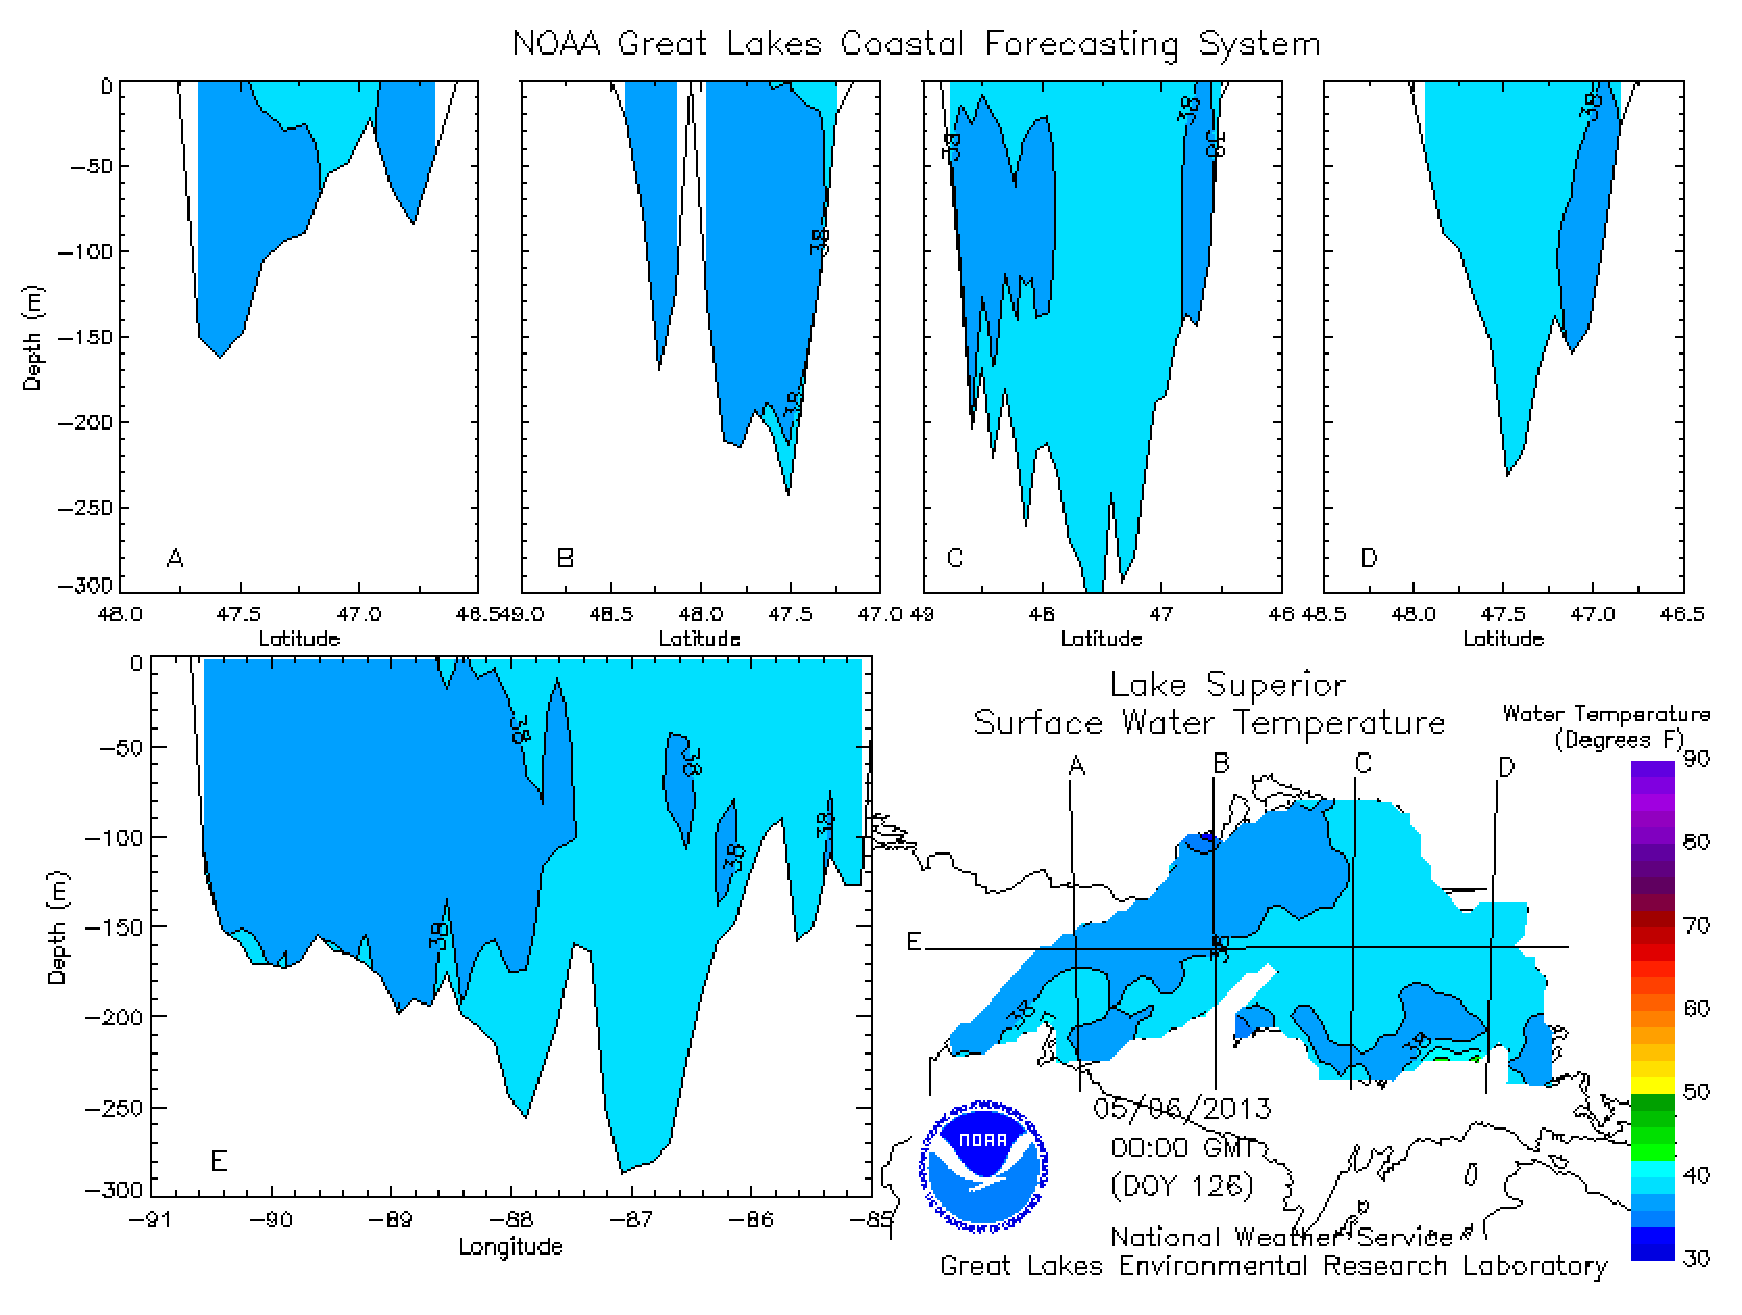
\includegraphics[width=5in]{figures/noaa.eps}
   \caption{Lake Superior water temperature transects (source: NOAA).}
   \label{fig:noaa}
\end{figure}

\begin{wrapfigure}{r}{0.45\textwidth}
   \centering
   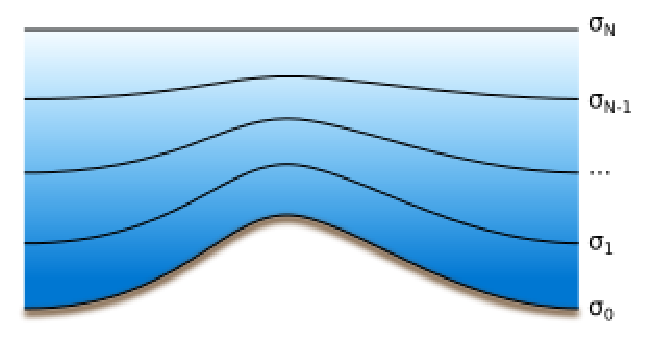
\includegraphics[width=2in]{figures/sigma.eps}
    \caption{A sigma vertical coordinate system (source: Wikipedia).}
   \label{fig:sigma}
\end{wrapfigure}

Great Lake Operational Forecast System (GLOFS) output files are released hourly by NOAA, featuring nowcoast and forecast guidance out to thirty hours, though we ignored the time dimension.  For each of the five Great Lakes, GLOFS uses a separate configuration of the Princeton Ocean Model (POM) \cite{pom}.  POM is a numerical model used to simulate and predict ocean parameters.  It uses curvilinear coordinate grids, a free surface, and a sigma coordinate system to represent the vertical dimension.  Sigma coordinate systems follow the bathymetry of the ocean or lake bottom at evenly spaced depths, as shown in Figure \ref{fig:sigma}.

Our application was developed so that any of the five Great Lakes could be rendered by our application, but in particular we used Lake Superior for development and testing.  Lake Superior's version of POM features 61 by 30 grid cells about 10 kilometers across and 20 sigma layers.  We focused on using only the closest nowcast, since nowcasts tend to be more accurate than forecasts further in the future.

\subsection{NetCDF}

Network Common Data Form (NetCDF) by UCAR is an open standard, platform-independent format for storing array-oriented scientific data \cite{netcdf}.  Values in NetCDF are accessed by using temporal and/or spatial indices into the appropriate variable array.  UCAR also provides libraries to process NetCDF files, including a Java library.  The use of this Java library was necessary for our application because the NetCDF reader built into VTK was completely undocumented.

\subsection{Visualization Toolkit}

Visualization Toolkit (VTK) is an open-source, 3D computer graphics software system for visualization created by Kitware.  Designed and implemented using an object-oriented approach, VTK produces visualizations for exploring, transforming, and viewing data \cite[p. 5]{vtkGuide}.  It is the underlying software of KitWare's ParaView; using VTK directly provides for much more user control.  Though written in C++, it can be used in Java thanks to interpreted interface layers.  VTK was used in Java to handle the rendering, which would have been complex to implement from scratch.

\section{Project Description}

A Java application was developed to display interactive isosurfaces of a user-specified NetCDF file according to a color table and a configuration describing the NetCDF file.  Since this application was built using VTK, the user must have VTK installed on their machine with Java wrapping.  Additionally, the user must also have the NetCDF Java library available.

\subsection{Functionality}

After the user starts the application, two windows appear: (1) the rendering window where the isosurfaces are displayed and (2) the graphical user interface controls.  The controls allow the user to adjust what is displaying and how, while the user can adjust the view in the rendering window with different mouse actions.

\subsubsection{Configurations}

The user runs the program by specifying the NetCDF file to be processed, as well as a Java \code{Property} object that contains information about what the variable names in that specific NetCDF file.  Though this calls for slightly more work from the calling user, the use of the \code{Property} class allowed the program to be generalized so NetCDF files with slightly different variable names (e.g., ``lat" instead of ``latitude") could be processed the same.

\begin{wrapfigure}{r}{0.4\textwidth}
   \centering
   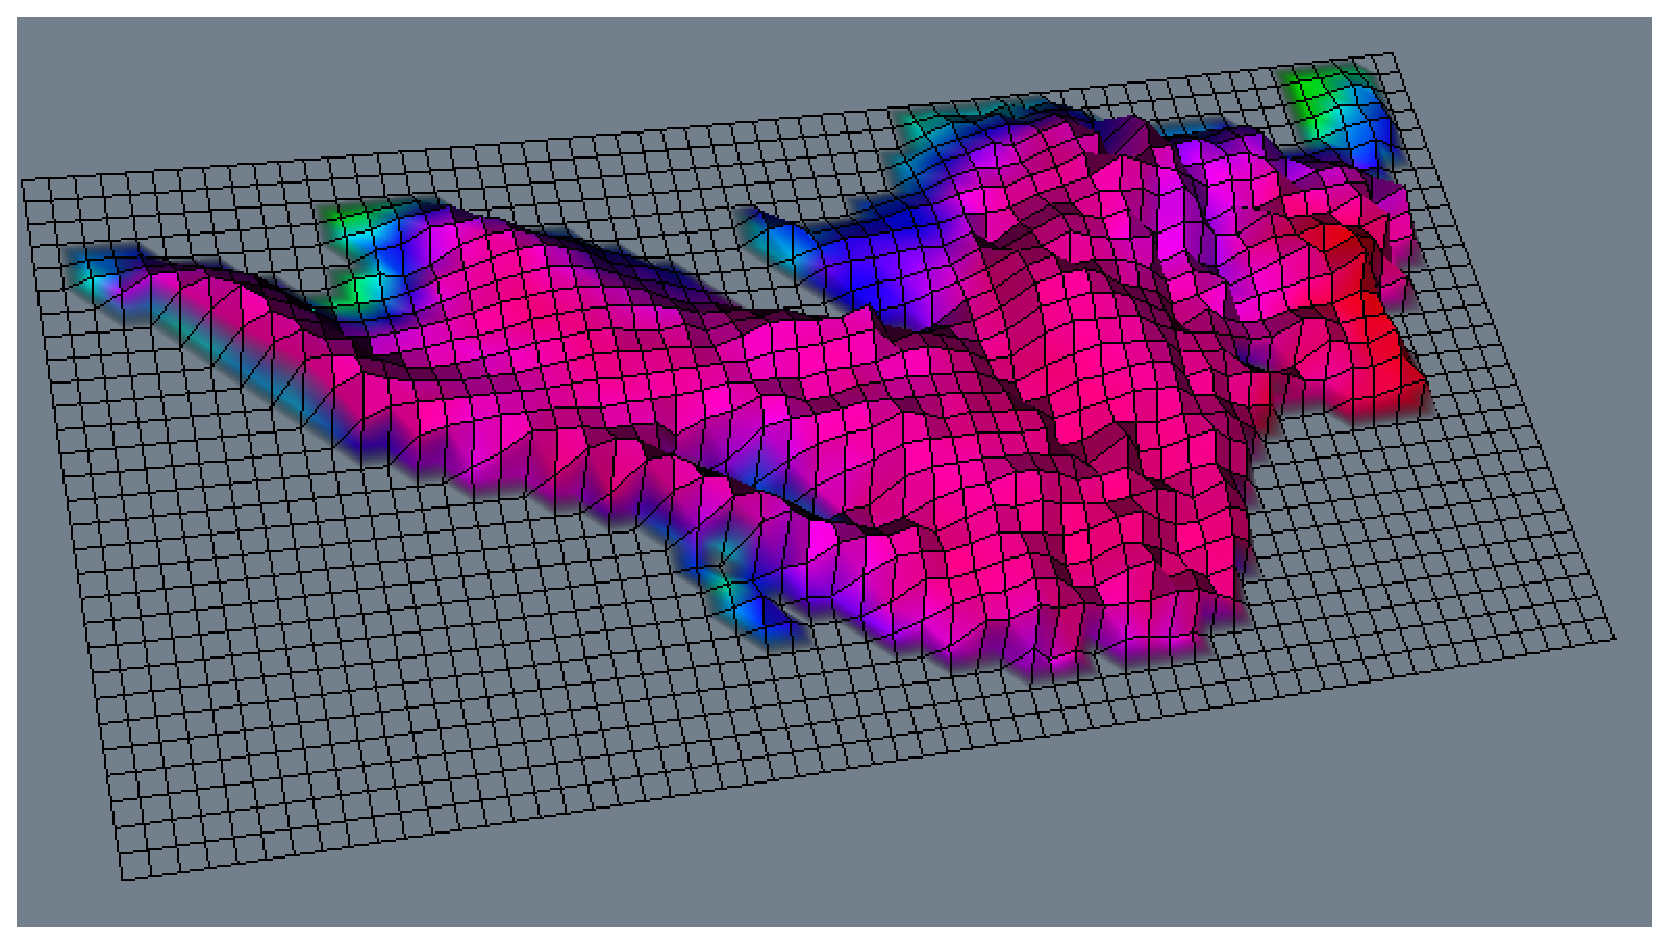
\includegraphics[width=1.8in]{figures/lakebelow.eps}
    \caption{Lake Superior, rendered as in ``full," rotated and viewed from below.}
   \label{fig:lakebelow}
\end{wrapfigure}

\subsubsection{Rendering Window}

We strove for simplicity with the rendering window, where VTK places actor objects.  Default lighting options were used, though user-defined lighting options could be configured in the future.  The user can interact with the actor(s) by rotating with the left mouse button, zooming with the right mouse button, and translating with the middle mouse button.  These mouse interactions are built into VTK.

The rotation action is useful for viewing the rendered volumes from multiple angles, which helps to understand the shape of the lake bottom.  Figure \ref{fig:lakebelow} shows Lake Superior after it has been rotated so it can be viewed from below.  Note that the visibility of the grid and the shading helps to provide insight on the curvature of the bathymetry.


\begin{wrapfigure}{r}{0.4\textwidth}
   \centering
   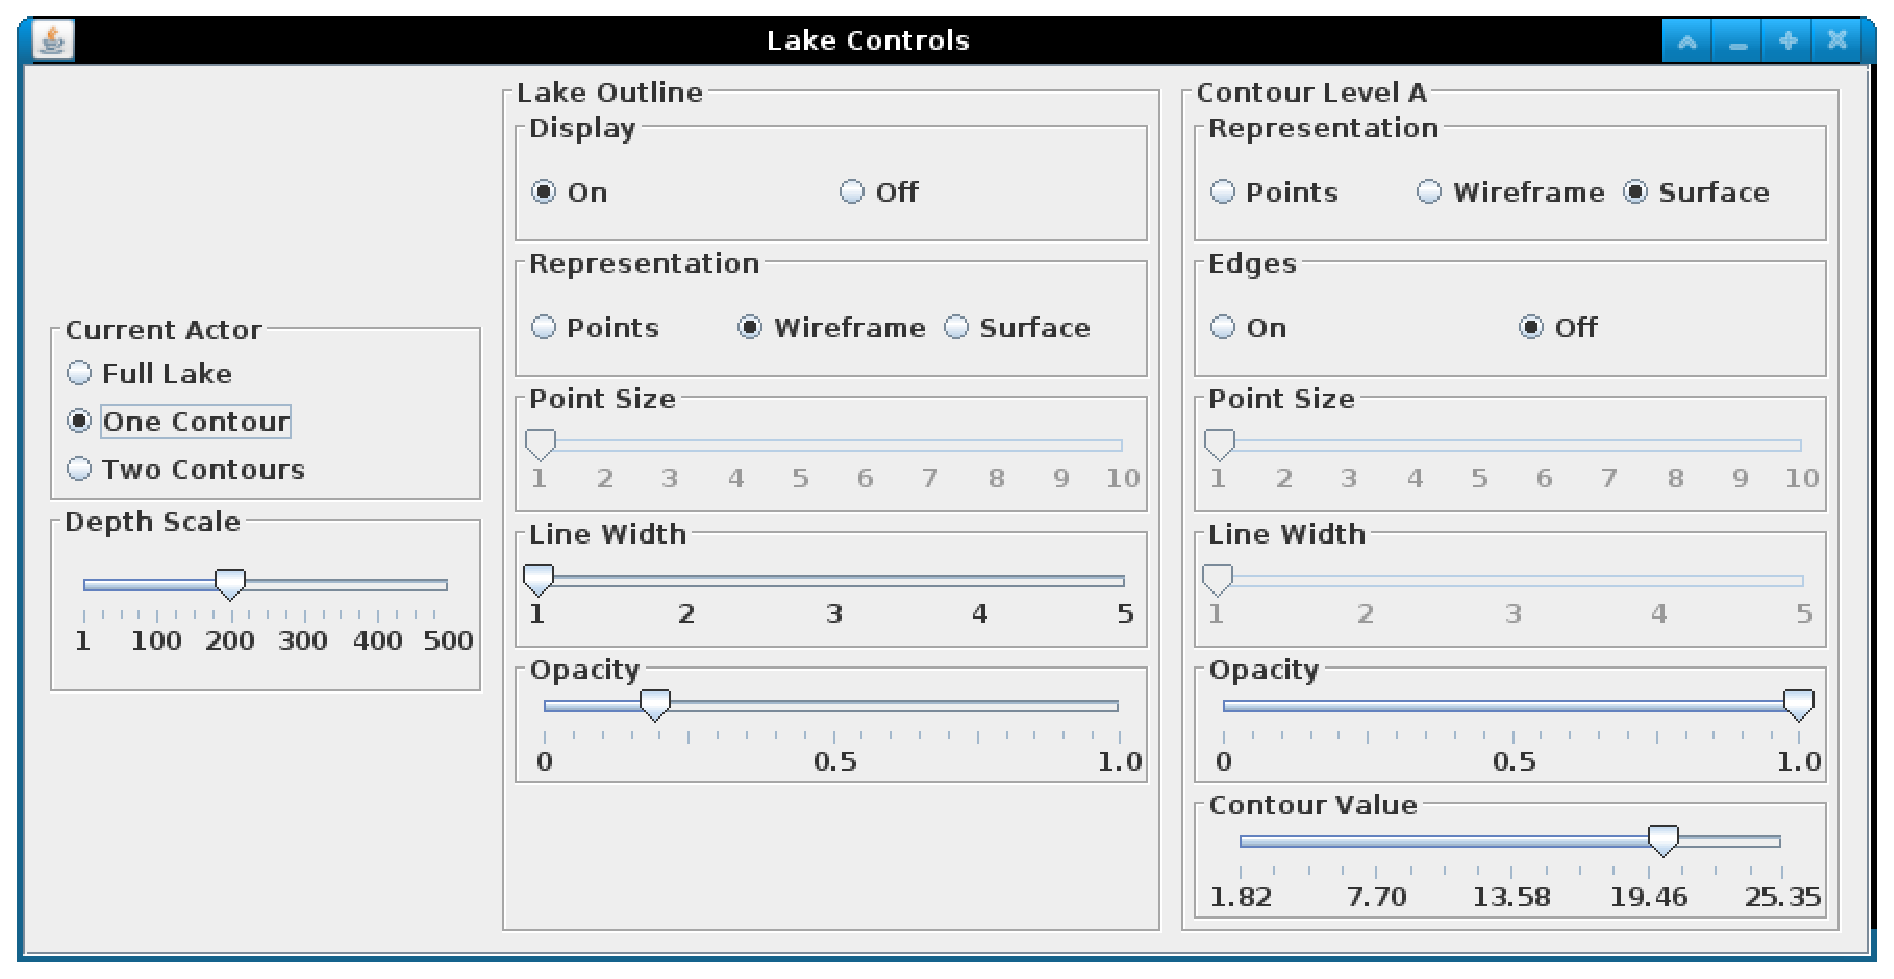
\includegraphics[width=1.8in]{figures/lakecontrols.eps}
    \caption{The user controls for the application.}
   \label{fig:controls}
\end{wrapfigure}


\subsubsection{Graphical User Interface Controls}\label{sec:gui}

The entire purpose of this isosurface rendering was to help a user gain understanding and insight into a Great Lakes OFS NetCDF file through interaction with the visualization.  Therefore, we knew we would have to develop a graphical user interface (GUI) which would provide controls for the user to transform the lake data.

Figure \ref{fig:controls} shows a screenshot of some of the controls available to the user for modifying and interacting with the volume rendering.  The options include the ability to render the ``full surface" (a sort of pseudo-isosurface featuring the water surface and bottom-most sigma layer fully colored for all temperature values, see Section \ref{sec:fullLake}), one contour, and two contours.  VTK refers to these objects as ``actors."  Optionally, a black ``boundary" of the entire lake can be turned on to give some perspective to the user, as shown in figure \ref{fig:frame} (see Section {sec:lakeBoundary}).


\begin{figure}[htb]
%\begin{wrapfigure}{r}{0.4\textwidth}
   \centering
   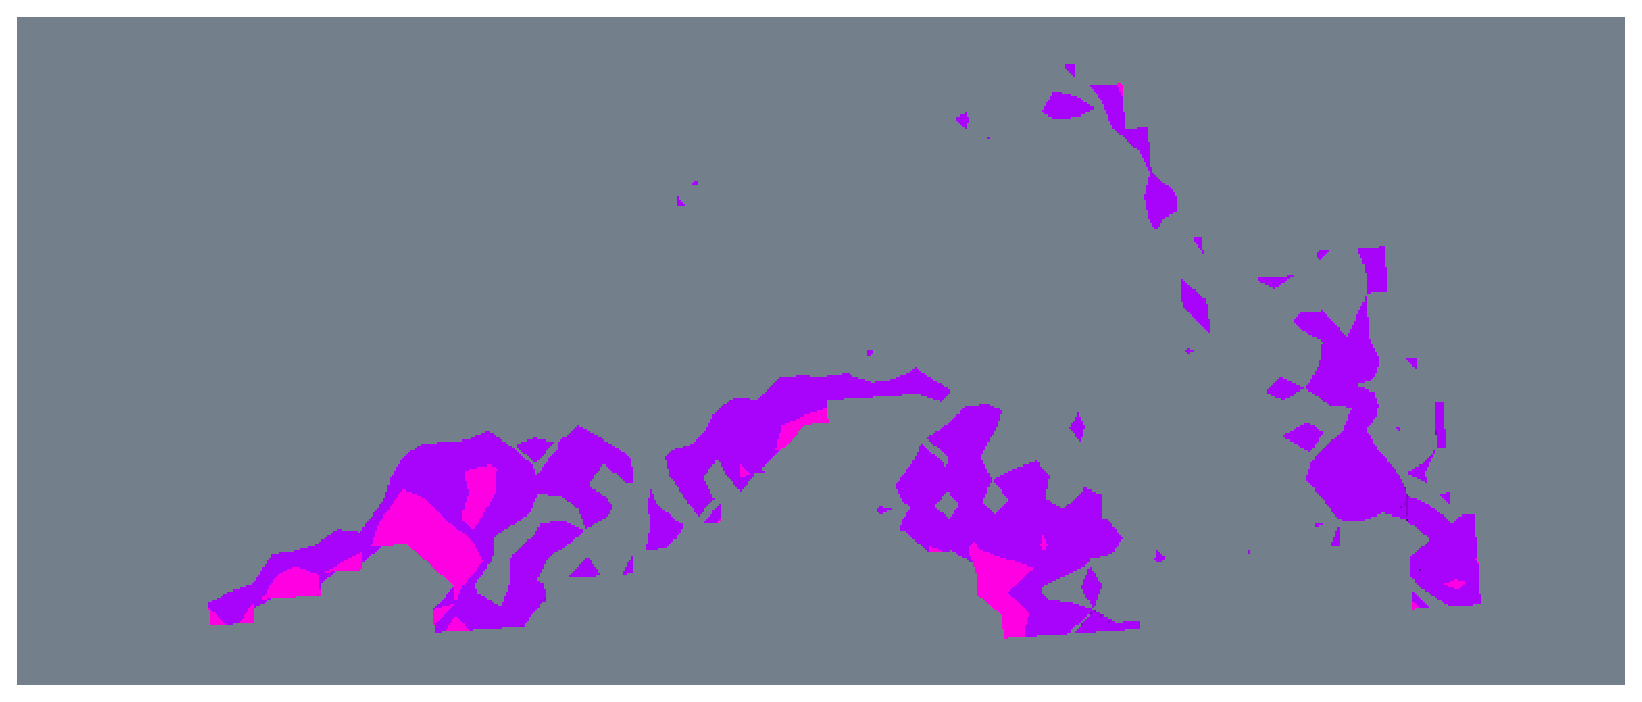
\includegraphics[height=0.85in]{figures/lakewithoutframe.eps}
   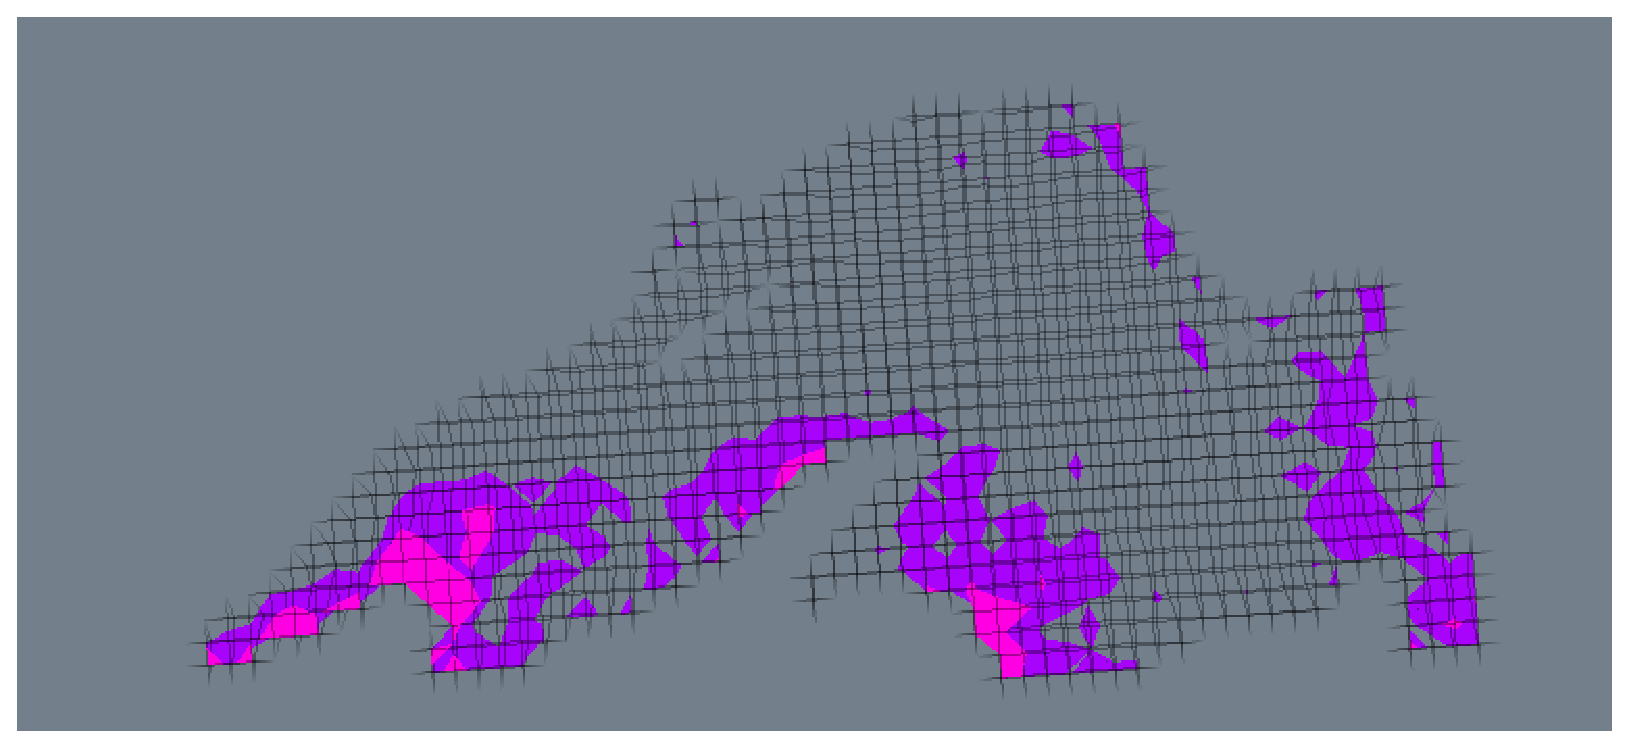
\includegraphics[height=0.85in]{figures/lakewithframe.eps}
    \caption{Two contour levels of Lake Superior, 18$^\circ$C in purple and 20$^\circ$C in pink, without and with the boundary of the lake.}
   \label{fig:frame}
%\end{wrapfigure}
\end{figure}

All types of actors and the boundary of the lake can be drawn as either a solid object, points, or a wireframe.  Independent controls exist for each actor to adjust the size of the points, the width of the wireframe lines, or the visibility of edges for the solid rendering. The opacity of each actor can also be individually controlled.

A slider can control the depth scale for all present actors, the results of which can be seen in Figure \ref{fig:vertscale}.  Without this slider, the Great Lakes appear to be completely flat, so it is necessary to scale the depth in order to see any variation.  Further justification for the need to scale as well as the implementation of the scaling is explained later in Section \ref{sec:coord}.

There are controls to interactively change the color table file used.  The color table spans from the minimum and maximum values found within the data, but there is a ``range slider" which allows the user to adjust the range of values that map to the color table.  Pressing the ``Snap to Data" button maps from the minimum and maximum values found in the data, as is used by default. A \code{vtkLookupTable} object is used to map the values to the colors in the color table file.  Color table files feature one color listed per line, with a color defined as red, green, and blue values from 0 to 255.

``Depth peeling" can allow for better rendering of transparent objects in VTK.  There is a checkbox to toggle this feature on and off, as the effectiveness of this feature depends on the user's OpenGL installation and graphics card.  When depth peeling is on, it slows the rendering, so it is off by default.

Finally, there are sliders to adjust the red, green, and blue values of the background color of the rendering window.  The default color is a grey that may need to be adjusted depending on the color table used.

\subsection{Approach}

%\begin{wrapfigure}{r}{0.4\textwidth}
\begin{figure}[htb]
\centering
% Define block styles
\tikzstyle{block} = [rectangle, draw, fill=blue!10,
    text width=10em, text centered, rounded corners, minimum height=2em]
\tikzstyle{line} = [draw, very thick, color=black, -latex']

\begin{tikzpicture}[node distance = 1cm, auto]
    % Place nodes
    \node [block] (netcdf) {NetCDF file};
    \node [block, below of=netcdf] (floatsA) {floats $(lon, lat, alt)$};
    \node [block, below of=floatsA] (floatsB) {floats $(x, y, z)$};
    \node [block, below of=floatsB] (points) {\code{vtkPoints}};
    \node [block, below of=points] (grid) {\code{vtkStructuredGrid}};
    \node [block, below of=grid] (cf) {\code{vtkContourFilter}};
    \node [block, below of=cf] (map) {\code{vtkPolyDataMapper}};
    \node [block, below of=map] (act) {\code{vtkActor}};
    % Draw edges
    \path [line] (netcdf) -- (floatsA);
    \path [line] (floatsA) -- (floatsB);
    \path [line] (floatsB) -- (points);
    \path [line] (points) -- (grid);
    \path [line] (grid) -- (cf);
    \path [line] (cf) -- (map);
    \path [line] (map) -- (act);
\end{tikzpicture}
\caption{NetCDF to VTK pipeline.}
\label{fig:flowchart}
\end{figure}
%\end{wrapfigure}

Figure \ref{fig:flowchart} describes the general pipeline used for processing the NetCDF files and producing a renderable object in VTK.  We began by processing the individual variables in the file and converting them to Java \code{float} arrays.  Next, we converted the coordinate variables into points that share a common unit, kilometers.  From this, we ultimately built a \code{vtkStructuredGrid} object, which was the input for a \code{vtkContourFilter} that mapped to a \code{vtkActor}.  These steps are described in further detail below.

\subsubsection{NetCDF Parsing}

The usage of the \code{vtkNetCDFReader} class was unclear, so we used UCAR's NetCDF Java library to open and read the NetCDF files.  We developed a tool which would read a generic NetCDF variable and return an array of \code{float}s with the same dimensions as the original NetCDF variable.  This tool was made to be as general as possible so it could easily process all Great Lakes OFS files, which have different grid sizes, or potentially other NetCDF files without any issues.  It was crucial to ensure that the dimension sizes of the returned arrays matched the original in the NetCDF file, since later on \code{vtkStructuredGrid} needed to know the size of the dimensions in order to infer the connections between points.

\subsubsection{Coordinate Conversion}
\label{sec:coord}

VTK expects that all coordinate values are of the same unit.  This presented a problem because the coordinates in the NetCDF files -- longitude, latitude, zeta, depth, and sigma -- feature several coordinate systems.  Longitude and latitude are measured in degrees for each point $(i, j)$.  Zeta ($\zeta$) represents the time-varying free surface at a point and time $(i, j, t)$ and is in meters, with positive matching with the upward direction.  Depth ($d$), which is the unperturbed water column height at a given grid point $(i, j)$, is also measured in meters, but with positive going down.  The sigma variable ($\sigma$) describes what percentage of the full depth a sigma layer $s$ is.

Therefore, the actual altitude $alt$ in meters for a grid point $(i, j)$ at sigma level $s$ and at time $t$ is:

\begin{equation}\label{eq:depth}
alt(i, j, s, t) = [\zeta(i, j, t) - d(i, j))] \cdot \sigma(s)
\end{equation}

We used $t = 0$ for all files we processed, so this equation was simplified further:

\begin{equation}
alt(i, j, s) = [\zeta(i, j) - d(i, j))] \cdot \sigma(s)
\end{equation}

\begin{figure}[htb]
   \centering
%   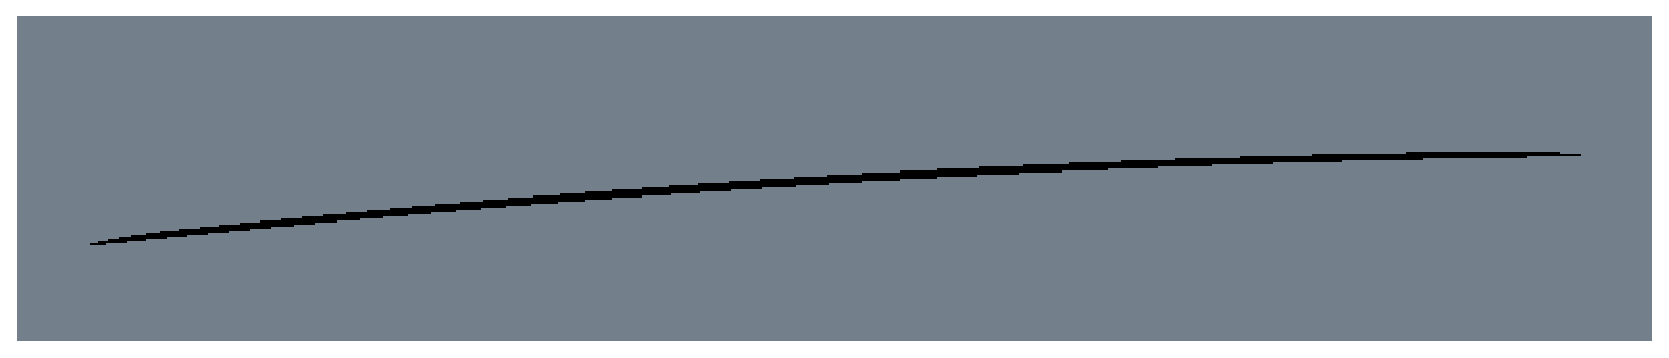
\includegraphics[scale=0.5,bb=0 0 785 156]{figures/vertscale1.eps}
   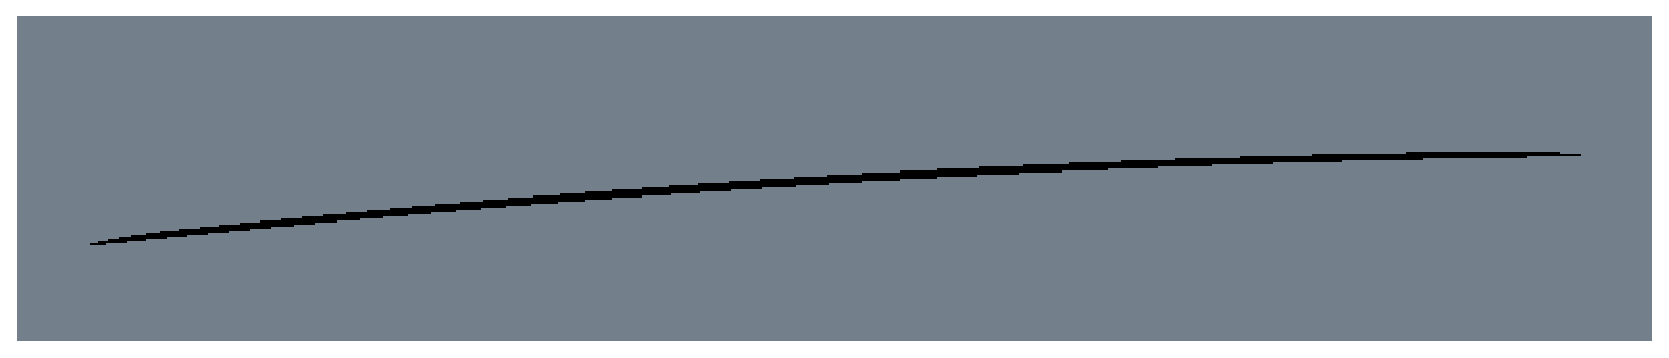
\includegraphics[width=4in]{figures/vertscale1.eps}
   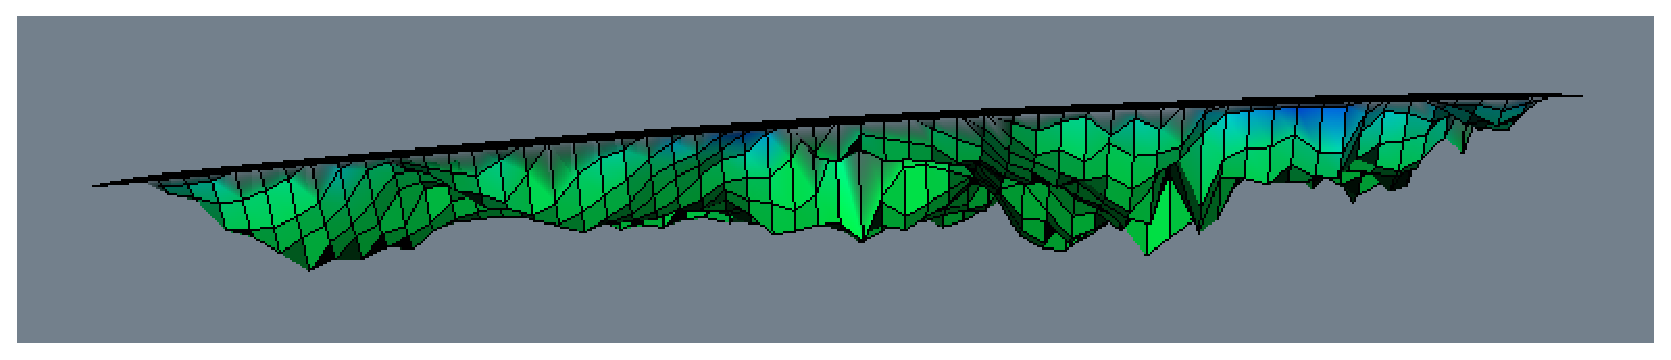
\includegraphics[width=4in]{figures/vertscale200.eps}
   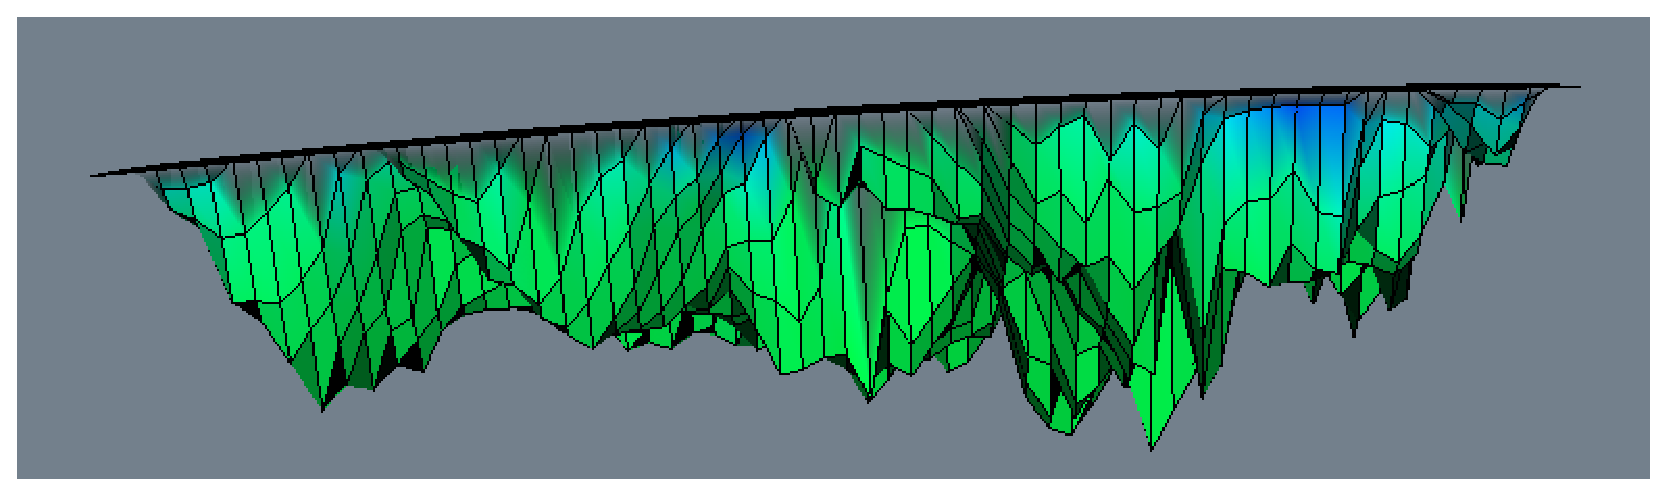
\includegraphics[width=4in]{figures/vertscale500.eps}
   \caption{Lake Superior with vertical scale factors of 1, 200, 500.}
   \label{fig:vertscale}
\end{figure}

The Great Lakes are quite shallow in comparison with their surface length and width.  To illustrate this, the curvilinear grid for Lake Superior is about 610 by 300 kilometers, while the lake is only 0.406 kilometers deep at its deepest point.  In other words, the grid is about 1500 times wider than the lake's deepest point.  To aid in the visualization, we decided to add a vertical scaling factor ($S \ge 1$) to the altitude calculation, as seen in use in Figure \ref{fig:vertscale}:

\begin{equation}\label{eq:finalAlt}
alt(i, j, s) = [\zeta(i, j) - d(i, j))] \cdot S \cdot \sigma(s)
\end{equation}

With this calculation done for each point $(i, j)$ at each sigma level $s$, we had $(lon, lat, alt)$ for every $(i, j, s)$.  This allowed us to do a conversion from $(lon, lat, alt)$ to Earth-Centered, Earth-Fixed (ECEF) $(x, y, z)$ values in meters.  ECEF is a Cartesian coordinate system where $(0, 0, 0)$ is defined as the center of the Earth \cite{geodesy}.  Each $(x, y, z)$ value could be added to a \code{vtkPoints} object, which was used to build a \code{vtkStructuredGrid}.

\subsubsection{Contour Filtering}

VTK provides who classes which are capable of scalar contouring as is necessary for isosurface rendering: \code{vtkContourFilter} and \code{vtkMarchingCubes}.  The former generates point, line, and surface contouring primitives depending on the input cell types; the latter generates primitives for structured points.  Since we built a \code{vtkStructuredGrid}, we initially attempted to use the \code{vtkMarchingCubes} technique.  Furthermore, when \code{vtkMarchingCubes} is a possible option, it is said to outperform \code{vtkContourFilter} by a factor of 1.4 to 7 \cite[p. 181]{vtkGuide}.

Unfortunately, the \code{vtkMarchingCubes} class would not work with our approach, so we used the \code{vtkContourFilter} technique instead.  Though this approach is slower, our application did not suffer and operates at interactive speeds.  This may be explained by the low resolution of the original NetCDF input file.  With larger files, the \code{vtkMarchingCubes} option should be further explored.

\subsection{Detailed Specification}

Provided below are low-level descriptions of some of the processes and decisions involved in this application.

\subsubsection{Dimension Ordering}

When we extracted Java \code{float} arrays from the NetCDF variables, we made every attempt to keep the data ordered in the same axis ordering with the same dimension sizes.  The variables in the NetCDF files were indexed by $(time, sigma, y, x)$.  Our code was implemented in a generalized manner so the dimensions can vary in size without a problem.  This was verified by testing the various Great Lake files, as they feature differently-sized grids.  However, we did not have any inputs to test different axis ordering (i.e., $(x, y, sigma, time)$), so behavior on files featuring alternative axis ordering is not guaranteed. 

\subsubsection{``Full Surface" Rendering}\label{sec:fullLake}

\begin{figure}[htb]
   \centering
   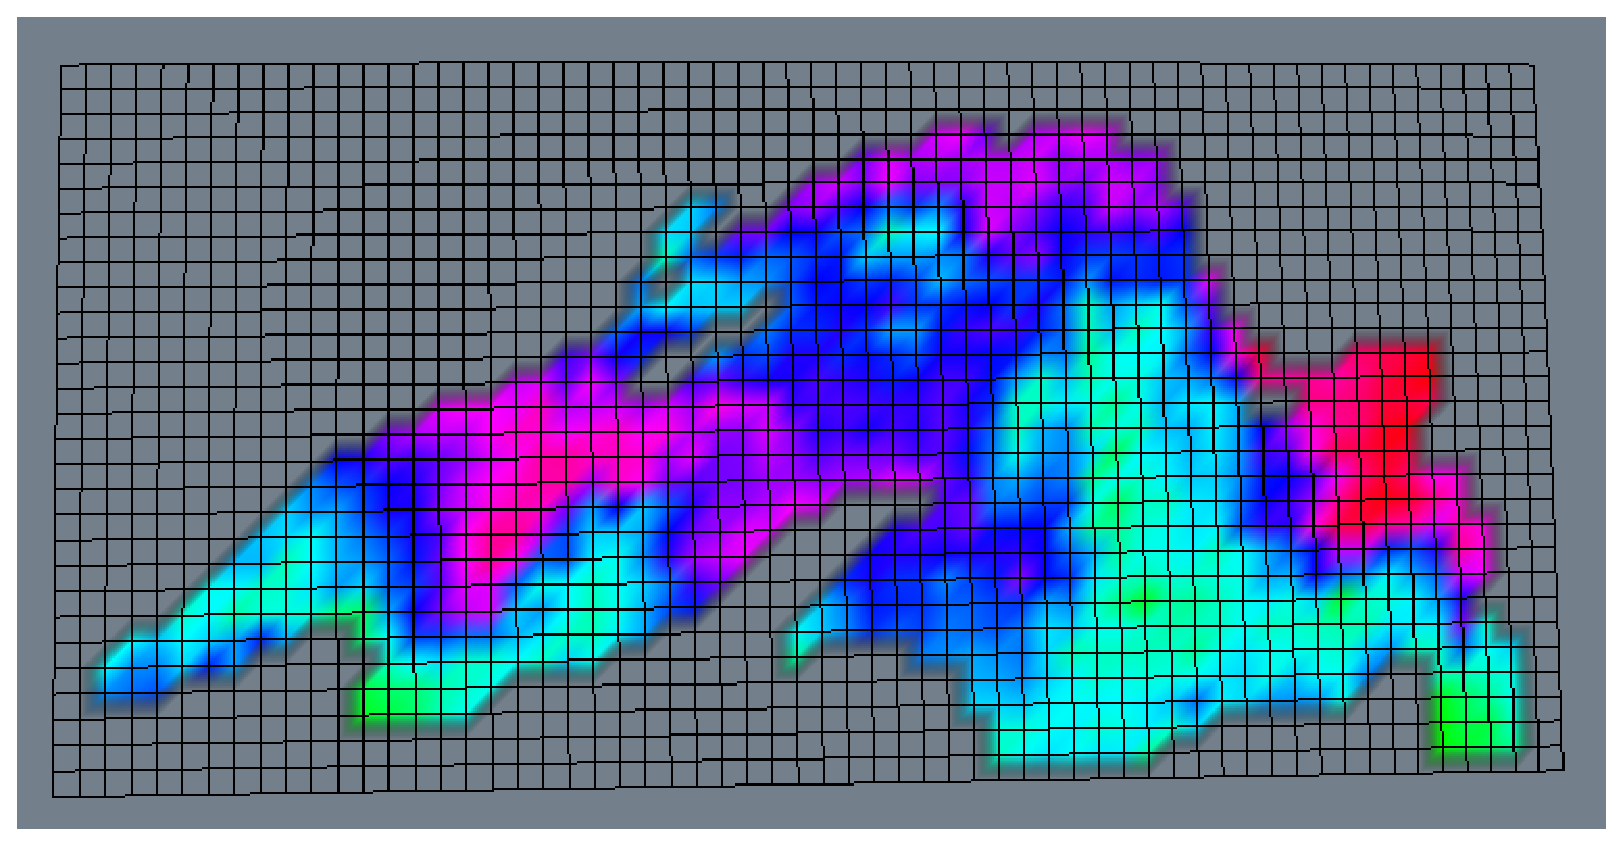
\includegraphics[width=4in]{figures/lakeabove.eps}
   \caption{``Full" Lake Superior, viewed from above.}
   \label{fig:lakeabove}
\end{figure}

Figures \ref{fig:lakebelow} and \ref{fig:lakeabove} show a sort of pseudo-isosurface rendering we have referred to as the ``Full Surface" rendering.  This is a rendering of the volume showing the surface and bottom-most sigma layer of the lake.  Each point of the surface is colored using a color scale spanning from the minimum and maximum values in the data.  A true isosurface only displays contours for a single scalar value, so by definition this is not a real isosurface.  However, it is interesting both to view by itself and to compare with the real isosurfaces, so we included this feature in the final application.  Figure \ref{fig:flowchartFull} shows the pipeline for this process, which is the same for the boundary actor.

%\begin{wrapfigure}{r}{0.4\textwidth}
\begin{figure}[htb]
\centering
% Define block styles
\tikzstyle{block} = [rectangle, draw, fill=blue!10,
    text width=10em, text centered, rounded corners, minimum height=2em]
\tikzstyle{line} = [draw, very thick, color=black, -latex']

\begin{tikzpicture}[node distance = 1cm, auto]
    % Place nodes
    \node [block] (netcdf) {NetCDF file};
    \node [block, below of=netcdf] (floatsA) {floats $(lon, lat, alt)$};
    \node [block, below of=floatsA] (floatsB) {floats $(x, y, z)$};
    \node [block, below of=floatsB] (points) {\code{vtkPoints}};
    \node [block, below of=points] (grid) {\code{vtkStructuredGrid}};
    \node [block, below of=grid] (map) {\code{vtkDataSetMapper}};
    \node [block, below of=map] (act) {\code{vtkActor}};
    % Draw edges
    \path [line] (netcdf) -- (floatsA);
    \path [line] (floatsA) -- (floatsB);
    \path [line] (floatsB) -- (points);
    \path [line] (points) -- (grid);
    \path [line] (grid) -- (map);
    \path [line] (map) -- (act);
\end{tikzpicture}
\caption{NetCDF to VTK pipeline for full surface and boundary.}
\label{fig:flowchartFull}
\end{figure}
%\end{wrapfigure}

\subsubsection{Lake Boundary}\label{sec:lakeBoundary}

\begin{figure}[htb]
   \centering
   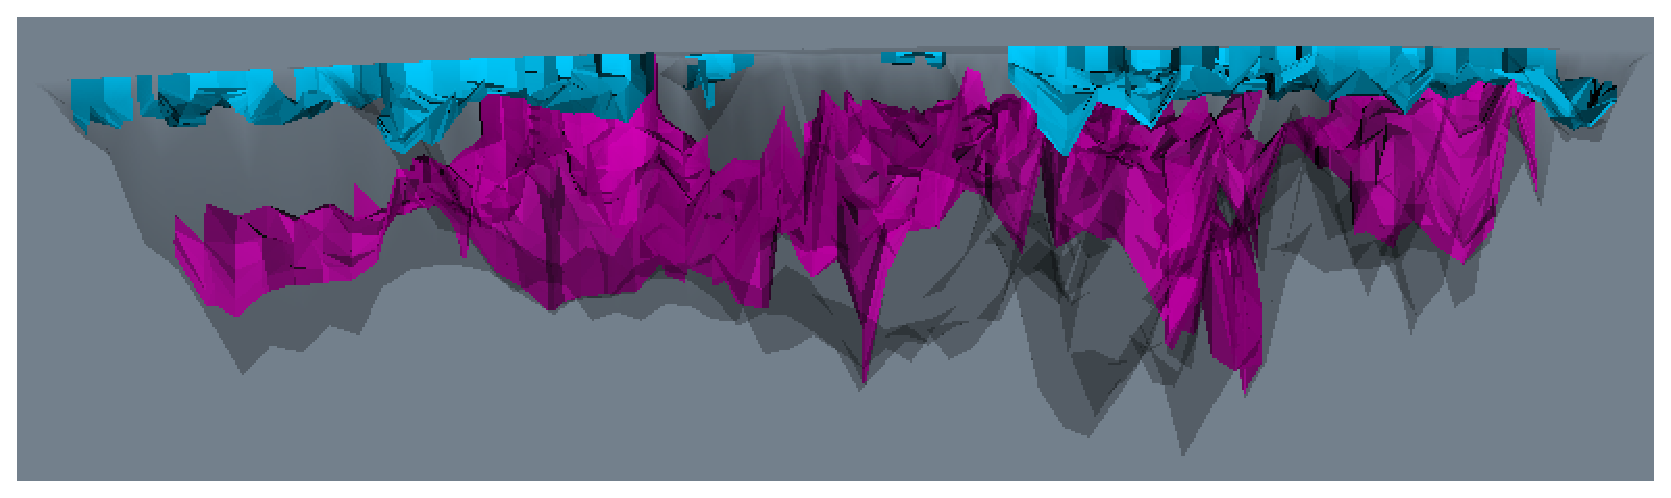
\includegraphics[width=4in]{figures/lakeside.eps}
   \caption{Two contour levels in Lake Superior viewed from the side with the lake boundary visible.}
   \label{fig:lakeside}
\end{figure}

It is difficult to draw conclusions from the viewing of isosurfaces without perspective of where the isosurfaces lie in the lake as a whole.  Therefore, we included the ability to draw an boundary of the entire lake to add some context.  The visibility of this boundary can be easily toggled.  As mentioned in Section \ref{sec:gui}, the opacity is adjustable and the representation can be changed between point, wireframe, and surface.

The actor for this ``boundary" is exactly the same as the ``full surface" actor, but using a color table that features only black.  Thus, it is a rendering of the surface of the lake and the bottom-most sigma layer that has been colored in black for all temperature values.  Figure \ref{fig:flowchartFull} shows the pipeline for this process.   Figure \ref{fig:frame} shows a comparsion of an above view with and without the boundary, while Figure \ref{fig:lakeside} shows a side view of two isosurfaces with the boundary turned on.

\subsubsection{Vertical Scaling}

A scale transformation could not be applied to adjust the scaling of the depth of the lake, because the vertical scale factor is applied before the conversion from longitude, latitude, and altitude to ECEF coordinates, as shown in Figure \ref{fig:flowchart}.  Therefore, each time the control for the vertical scale factor is adjusted by the user, the application must recalculate the altitude value for each point, as shown in Equation \ref{eq:finalAlt}.  Then the pipeline as shown in Figure \ref{fig:flowchart} must be redone from the second level to produce a \code{vtkActor} for rendering.  The first level of the pipeline is not repeated, since the NetCDF file needs to be read only once.

The NetCDF files have low enough resolution that repeating these calculating and conversions still provides for interactive speeds.  Still, we attempted to allievate the process by creating a \code{HashMap} of \code{vtkStructuredGrid} objects, with the vertical scale factor as the key.  This approach would not be recommended if the original file is of a much higher resolution and/or limited memory is available.

\subsubsection{ECEF Conversion}

After finding no documentation indicating otherwise, we assumed that the datum for the longitude and latitude values was World Geodetic System 1984 (WGS 84).  WGS 84 is commonly used standard in cartography and navigation.  However, if documentation is found that indicates another datum was used, then the conversion code should be modified to account for this.

Our conversion to ECEF code was based on an open-source JavaScript application \cite{geodesy}.  The conversion uses the WGS 84 ellipsoid.  It makes calculations by considering the radius of the earth at the specific latitude involved.

\section{Results}

\begin{figure}[htb]
   \centering
   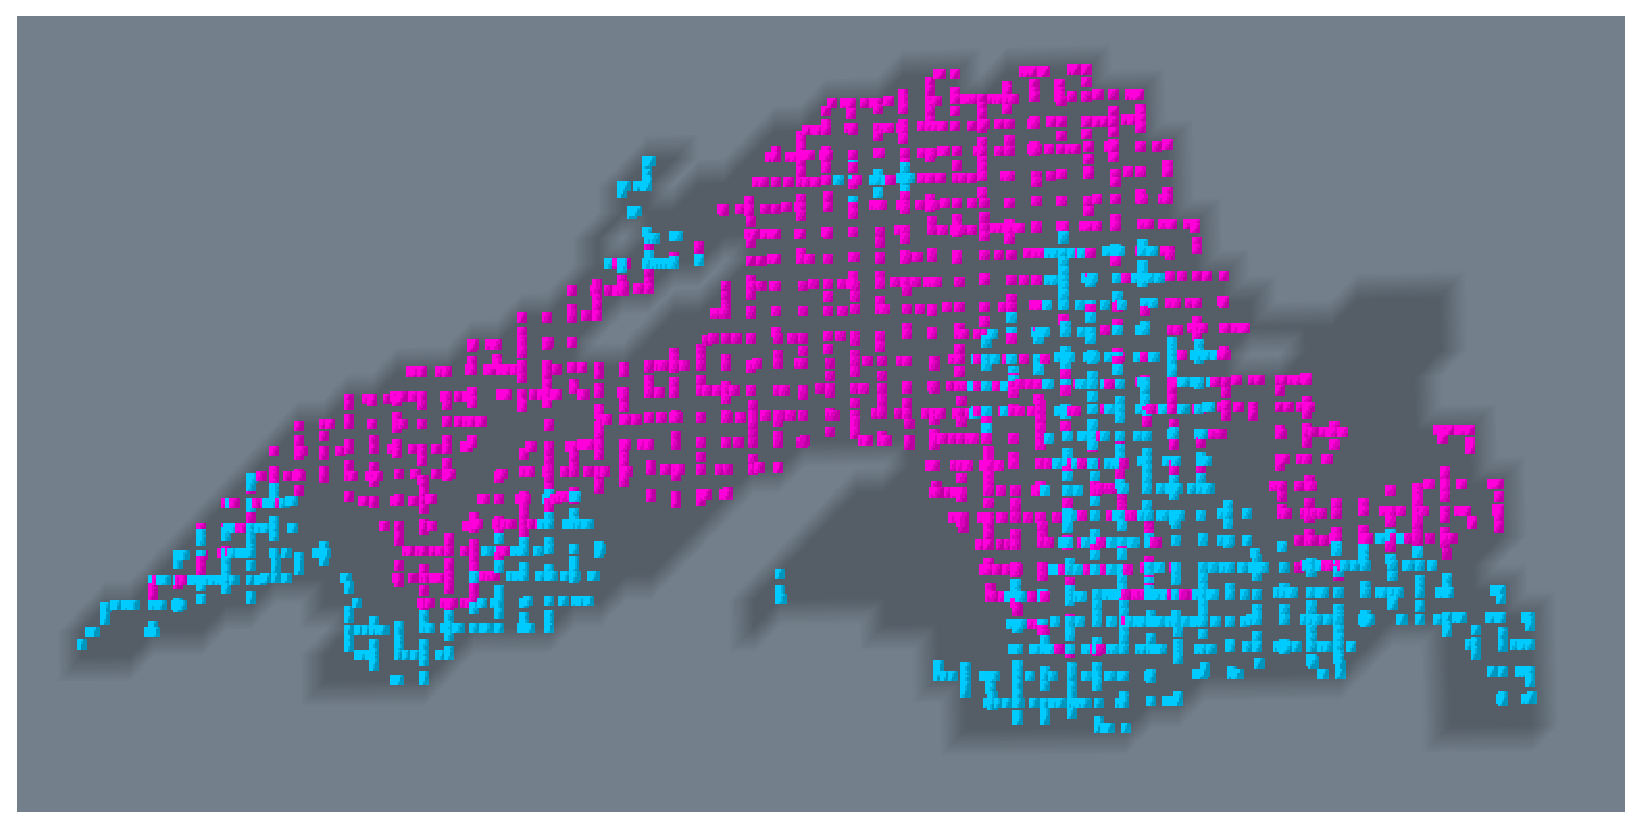
\includegraphics[width=3in]{figures/points.eps}
   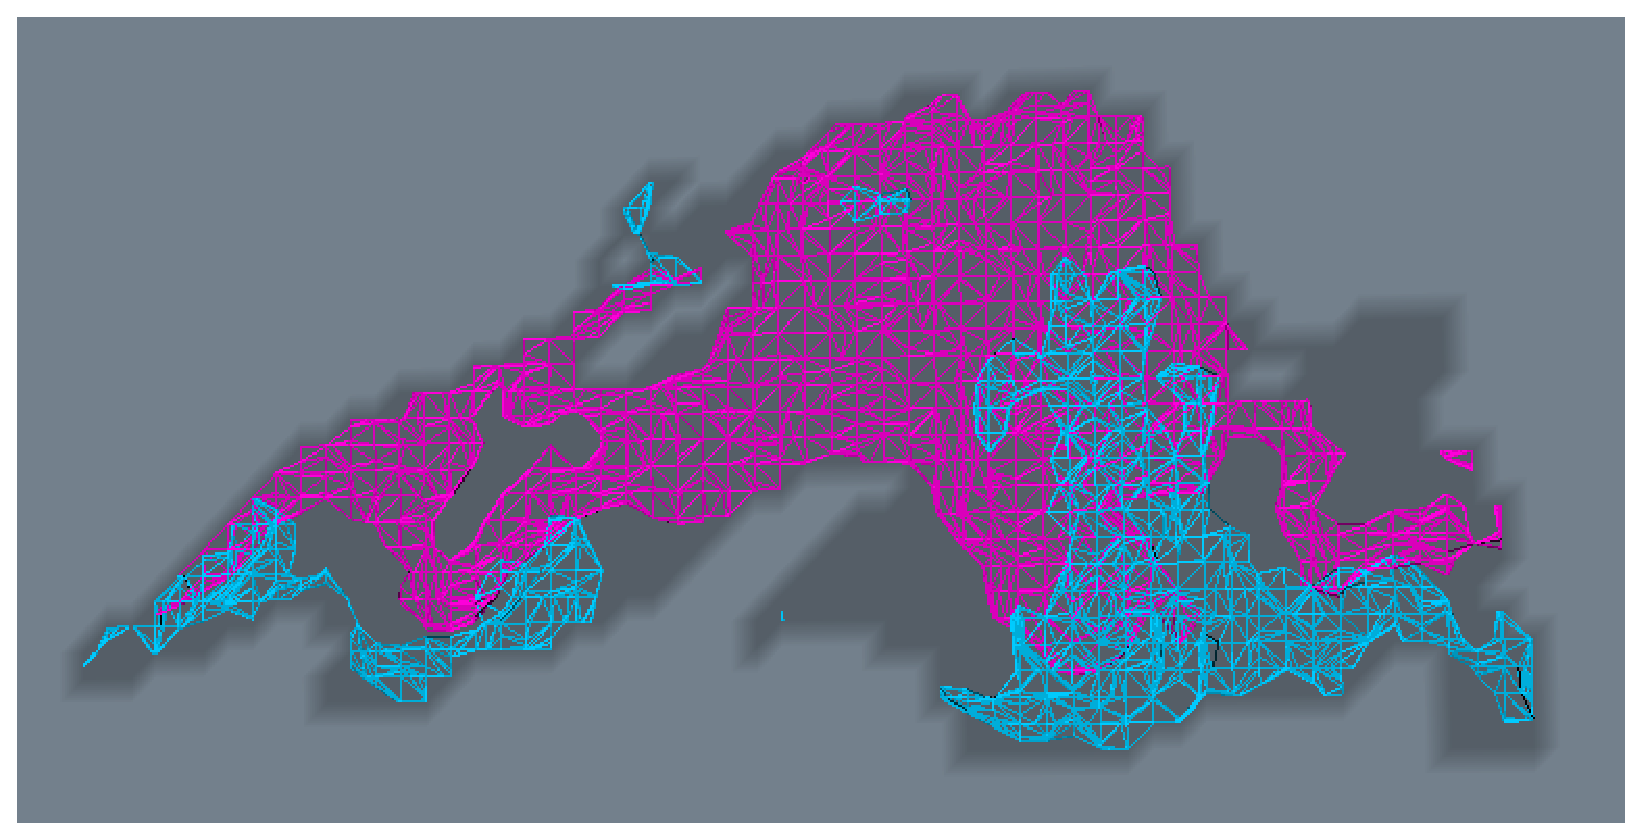
\includegraphics[width=3in]{figures/wireframe.eps}
   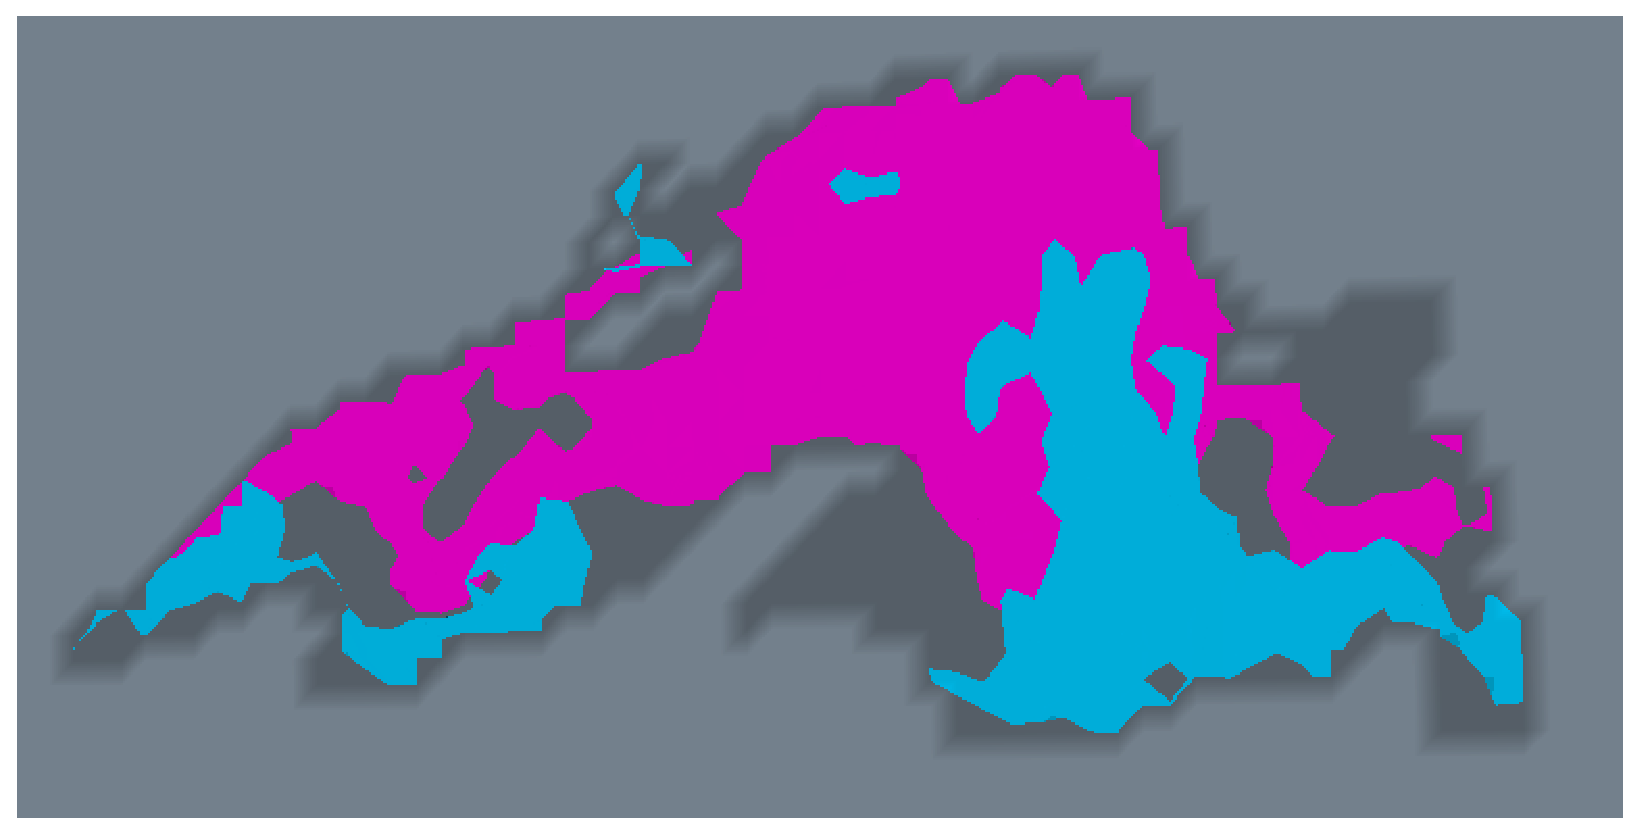
\includegraphics[width=3in]{figures/surface.eps}
    \caption{Two contour levels -- represented as points, wireframe, and solid objects -- of Lake Superior, seen from above.}
   \label{fig:rep1}
\end{figure}

Our application provides a lot of flexbility in viewing the water temperature of a Great Lake.  The user can easily select different isovalues, representations of isosurfaces, and more.  Figures \ref{fig:rep1} and \ref{fig:rep2} show the same contour levels, but with the different possible representations and from different views.  Representations can easily be mixed (e.g., one contour with points and another as a solid object) and changed.  Depth scales can be adjusted as in Figure \ref{fig:vertscale} and the lake boundary can be toggled as in Figure \ref{fig:frame}.  The controls are easy to understand for even new users.  

One downside to this application is VTK must be installed with Java wrapping to run it.  This is somewhat restrictive, as the installation of VTK is non-trivial on some platforms such as Windows.

\begin{figure}[htb]
   \centering
   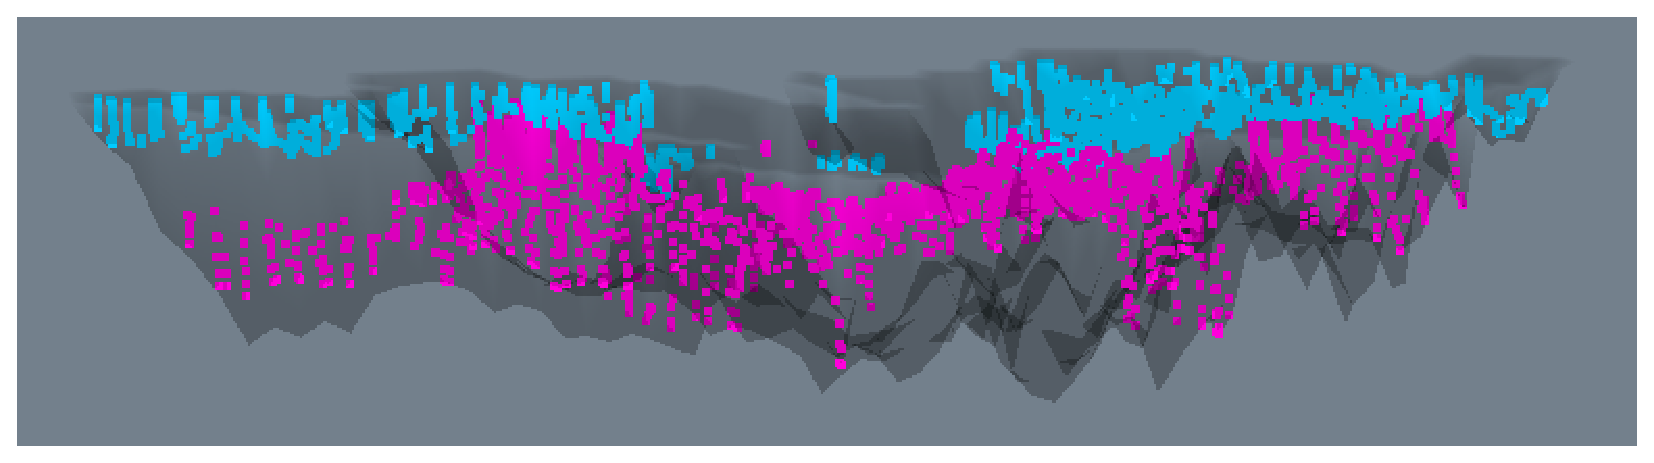
\includegraphics[width=4in]{figures/points2.eps}
   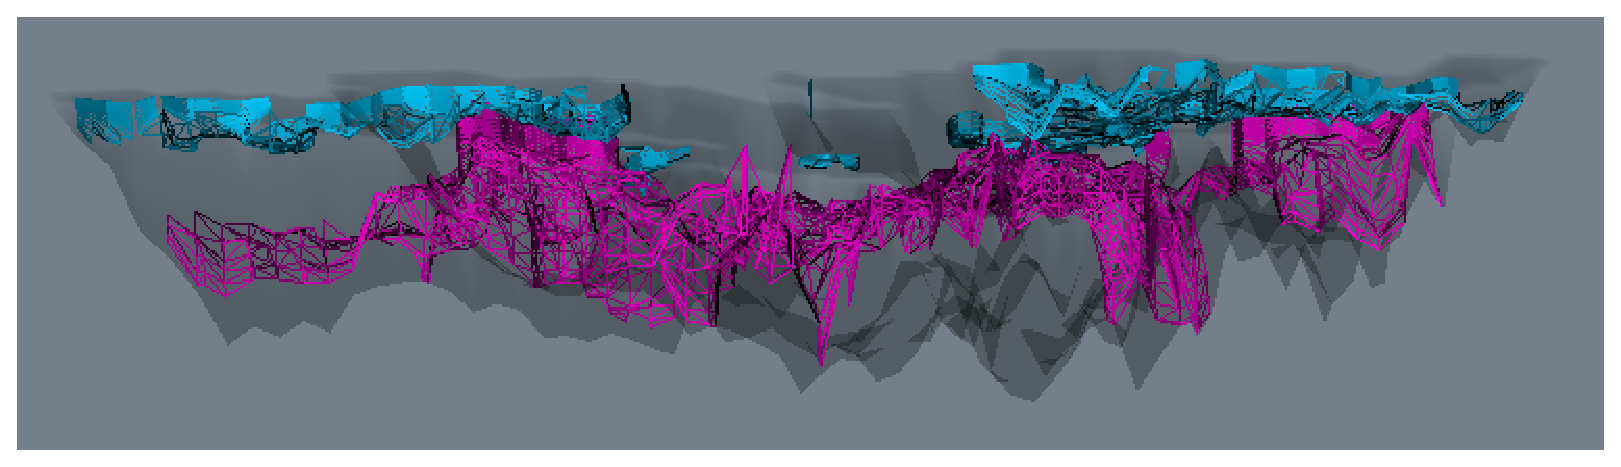
\includegraphics[width=4in]{figures/wireframe2.eps}
   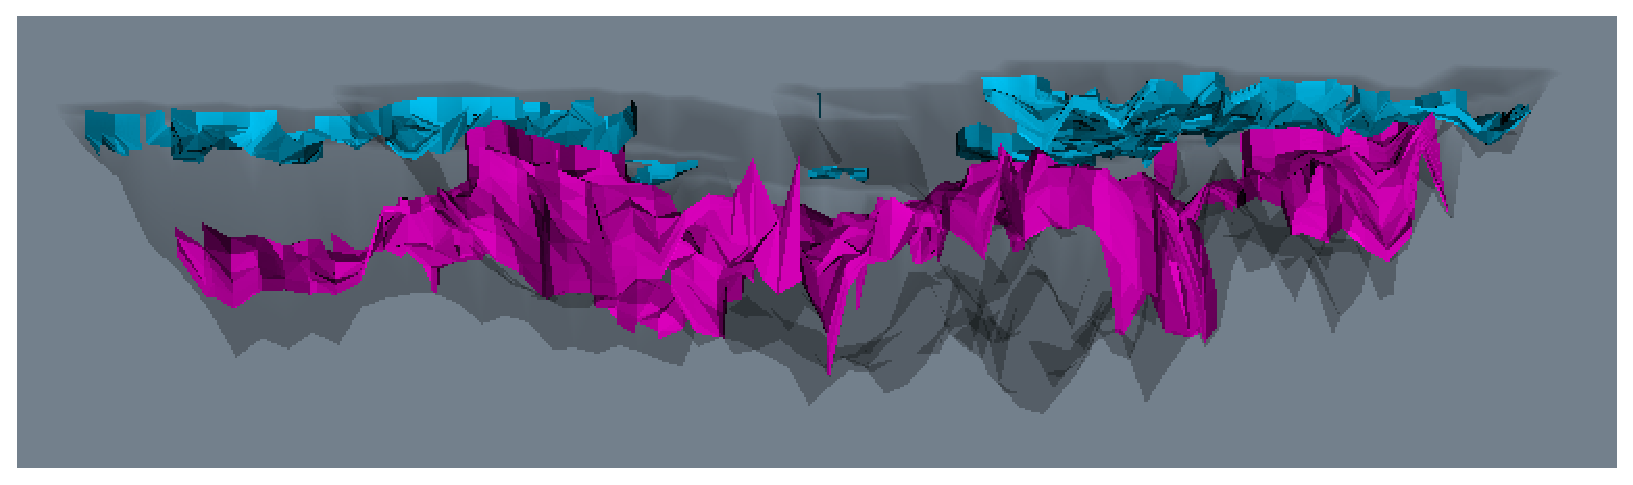
\includegraphics[width=4in]{figures/surface2.eps}
    \caption{Two contour levels -- represented as points, wireframe, and solid -- of Lake Superior, seen from the side.}
   \label{fig:rep2}
\end{figure}

\section{Conclusions}

The isosurface renderer we developed helps to interpret and understand the Great Lake Operational Forecast System NetCDF output files.  Users can easily gain insight to what water  temperatures seem to be where in the lake.  Other characteristics, such as where the temperatures are varying most, can also easily be inferred from the visualization.  The ability to change different viewing properties and transform the actors in the scene further enhance a user's understanding of the underlying data. This isosurface rendering application may be valuable for meteorologists and oceanographics, or perhaps even the original Great Lakes Operational Forecast System modelers.

\subsection{Future Steps}

There are limitless possibilities for additions to this application.  Some simple ones include the ability for the user to view more than two isosurfaces at once, control clipping planes, and control lighting.

\subsubsection{Portability}

In the future, it would be nice to have a more portable version of this program.  This could be accomplished perhaps by writing isosurface extraction and rendering code ``from scratch" using OpenGL or some similar program.  Another possibility would be to explore writing the program in C++ or Tcl, which do require VTK installations as well but no wrapping, so those languages may prove to have more slightly portable results. 

\subsubsection{Web Application}

Ultimately, if this application could be integrated into a browser, then this might be something which NOAA could display on their own website.  Currently, NOAA only features still images transects from predefined, static location, as seen in Figure \ref{fig:noaa}.  Our application proved to be very fast and might be fast enough for online purposes, though this would need to be further investigated.

\subsubsection{Other Input Data}

NOAA provides Operational Forecast System data for various regions, such as Chesapeake Bay, Northern Gulf of Mexico, and Delaware Bay.  These files are of a much higher resolution and feature more complex depth equations than the equations needed for the Great Lakes (Equation \ref{eq:depth}).  It would be interesting to extend our application to handle these files and see how it scales to higher resolution input.

Furthermore, the ability to process additional file types beyond NetCDF should be an easy addition.

\bibliographystyle{plain}

\bibliography{carmen-isosurface-writeup}

%\nocite{*} 

\end{document}
